\chapter{Implementation}
This chapter will describe my implementation of the procedural road generation algorithm, how the roads produced here is integrated with the snow simulator with all the changes to the snow simulator this entails, and lastly it describes the details about my implementation of the USGS DEM to height map converter application.

\section{Procedural road generation}
For this project, I implemented the road generation algorithm described by \cite{roadgen} for generating a road through a terrain described by a discrete height map. The road generator is a separate program written in C++ implementing an A* search algorithm which takes in a terrain in form of a heightmap, and outputs a file in the RoadXML format (see \cite{roadxml}). This section will first present the particular A* implementation, then it will describe how the clothoid spline is generated. Lastly, the RoadXML export code is described.

\subsection{Implementation of A*}
An A* search often has a very large amount of insertion operations to the $OPEN$ set, as it is used in algorithm \ref{alg:astar}. In addition, every iteration the node with the lowest $f$-cost must be retrieved from this set. Using an unsorted list gives a constant insertion time, but a really bad lookup-time when searching for the node with the lowest $f$-cost of $O(n)$. In the other extreme, a sorted list gives constant lookup-time, but insertion takes $O(n)$ time. 

Instead, typically a min-heap is used. A min-heap has a constant lookup-time because the next element to be extracted is always on top, but in addition the element must be removed, which takes $O(lg(n))$ time. Insertion takes in theory $O(lg(n))$ time, but due to the structure of the heap, in practice this cost is constant on average. In this implementation, a min-heap is used. 
a
\subsubsection{Grid coarsening}
Typically in an A* search every grid point is used as a node in the graph. For huge maps, say $4096\times 4096$, this approach becomes very slow due to the complex cost function used for procedural road generation. A more complex cost function makes it harder to make a heuristic that is both efficient and accurate for the distance to the goal, which causes A* to expand more nodes, and thus scale poorly with larger problems. A solution to this is to coarsen the grid used, so that instead of using every elevation point in the heightmap as a node, we use every $m$ nodes, as shown in figure \ref{fig:grid_coarsening}. This significantly reduces the number of nodes, making it viable to create paths through larger terrains.

\begin{figure}[ht]
\centering
\subfloat[$m=2$]{\includegraphics[width=0.3\textwidth]{figure/grid_coarsening_m2}}
\qquad
\subfloat[$m=4$]{\includegraphics[width=0.3\textwidth]{figure/grid_coarsening_m4}}
\caption{Grid coarsening with grid points every 2 and 4 elevation point}
\label{fig:grid_coarsening}
\end{figure}

\subsubsection{Neighborhood mask creation}
A typical A* implementation for use with a grid like the discretization of a terrain often use eight neighbors. \cite{roadgen} propose that not only the immediate eight neighbors are used per node, but instead use a larger neighborhood as described in section \ref{sec:roadgen_shortestpath}, and as shown in figure \ref{fig:neighbormask}. 

The naive implementation of utilizing this would be to for each node loop over each neighboring node within a distance $k$, check if $gcd(i,j)=1$, and if so, compute the cost to that node and add it to the $OPEN$ list. This does a lot of uneccesary checks as many of those neighbors will not be selected for expansion because $gcd(i,j)\neq 1$. Instead, the neighborhood mask are precomputed before the search starts and put in an an array. This allows us to instead loop over the array, with exactly as many elements as there is neighbors that will actually be expanded. The pseudocode for the generation of neighborhood masks are given in algorithm \ref{alg:neighborhoodmask}.

\begin{algorithm}
\begin{algorithmic}
\STATE Let $M$ be the neighborhood mask, initially empty.
\FOR {$i := 0\to k$}
    \FOR {$j := 0\to k$}
        \IF {$gcd(i,j) \neq 1$}
            \STATE continue
        \ENDIF
        \STATE $M := M + (i,j)$
        \IF {$ i \neq 0$}
            \STATE $M := M + (-i,j)$
        \ELSIF {$j \neq 0$}
            \STATE $M := M + (i,-j)$
        \ELSIF {$i \neq 0 \land j \neq 0$}
            \STATE $M := M + (-i,-j)$
        \ENDIF
    \ENDFOR
\ENDFOR
\end{algorithmic}
\caption{Pseudocode for constructing the neighborhood mask}
\label{alg:neighborhoodmask}
\end{algorithm}

\subsection{Trajectory generation} 
A clothoid spline can be used to model the road trajectoy, as this gives smooth curves with linearly varying curvature. The method described in \cite{clothoid} is used (see section \ref{sec:back_clothoid}). A class {\texttt ClothoidPair} was written to take care of constructing each clothoid pair in the spline, while the class {\texttt ClothoidSpline} contains one or more clothoid pairs that makes up the spline.

\subsubsection{Constructing the clothoid spline}
After the control points have been generated by the A* search as described above, these are passed on to the ClothoidSpline constructor. This constructor will first determine the connection points ${\mbf p}_0, ..., {\mbf p}_n$, i.e. where the clothoid pairs begin and end; this is done as described in section \ref{sec:clothoid_spline}. The end points are used as connection points as well. These points are then removed from the control vertex list. The tangents are then determined as 
\begin{equation}
{\mbf T}_i = 
\begin{cases}
({\mbf v}_i - {\mbf p}_i)/||{\mbf v}_i - {\mbf p}_i||_2 & \mbox{if $i = 0$}\\
({\mbf p}_i - {\mbf v}_{i-1})/||{\mbf p}_i - {\mbf v}_{i-1}||_2 & \mbox{if $i > 0$}
\end{cases}
\label{eq:connector_tangents}
\end{equation}

The next step is to  construct a clothoid pair that begins and ends at the connecting vertices for each control vertex, such that the tangent of the clothoid at the endpoints are the same as the tangent for the endpoints themselves. 

If the control points and its corresponding connection points are colinear, we simply use a straight line between the points. Otherwise, note that the starting point of clothoids have a tangent of ${\mbf T} = (1,0)$ and position $(0,0)$; this means that the clothoids must be translated and rotated rotated  to coincide with the points and tangents at the end points. Note also that we do not need to rotate and translate the points themselves, only the final clothoids. 

In each clothoid pair, one clothoid must be flipped; this is because the clothoids have different signs on the derivative of their curvature; i.e. $Sgn(\frac{d\kappa_{0}}{dt})\neq Sgn(\frac{d\kappa_{1}}{dt})$.  To test for which clothoid needs flipping, it is sufficient to check the sign of the third component in the cross product ${\mbf g}\times {\mbf h}$ where ${\mbf g}$ and ${\mbf h}$ are the vectors representing the longest and shortest vectors, respectively, of ${\mbf v}-{\mbf P}_0$ and ${\mbf P}_1 - {\mbf v}$. If the sign is negative, the clothoid starting in ${\mbf P}_0$ must be flipped; otherwise, the other clothoid must be flipped.

Finally, the scaling factors $a_0$ and $a_1$, and the tangent angle deviation for the first clothoid at the meeting point $\theta_0$ are computed. Note that $\theta_1$ is computed using $\theta_1 = \alpha - \theta_0$ because $\theta_0 + \theta_1 = \alpha$\cite{clothoid}. $\theta_0$ is found by using Newton's method to solve equation \ref{eq:theta0equation} in section \ref{sec:clothoid_spline}. An intial guess of $x=\alpha/2$ is used, which is reasonable because $\theta_0$ is somewhere between $0$ and $\alpha$.\cite{clothoid}. The scaling factors is found by solving equation \ref{eq:a0equation} for $a_0$, also in section \ref{sec:clothoid_spline}. $a_1$ is found using the formula given in equation \ref{eq:a1equation}. The complete pseudocode for constructing the clothoid spline is seen in algorithm \ref{alg:clothoid_spline_construct}.

\begin{algorithm}[ht]
\centering
\begin{algorithmic}
\REQUIRE Control points $W=\{{\mbf v}_0, {\mbf v}_1, ..., {\mbf v}_n\}$
\REQUIRE Connection points $Q=\{{\mbf v}_0, ({\mbf v}_1+{\mbf v}_2)/2, ({\mbf v}_2+{\mbf v}_3)/2, ..., ({\mbf v}_{n-2}+{\mbf v}_{n-1})/2, {\mbf v}_n\}$
\REQUIRE Tangents $T_i$ according to equation \ref{eq:connector_tangents}
\FOR{$i := 1\to n-1$}
\STATE $C := $ new clothoid pair
\STATE ${\mbf P}_0 := \argmax_{{\mbf p}} \{||{\mbf v}_i-{\mbf p}_{i-1}||_2, ||{\mbf v}_i-{\mbf p}_i||_2\}$
\STATE ${\mbf P}_1 := \argmin_{{\mbf p}} \{||{\mbf v}_i-{\mbf p}_{i-1}||_2, ||{\mbf v}_i-{\mbf p}_i||_2\}$
\IF{${\mbf P}_0, {\mbf v}_i, {\mbf P}_1$ is colinear}
\STATE $C.length := C.|S| := ||{\mbf P}_1 - {\mbf P}_0||_2$
\STATE $C.t_0 := C.t_1 := 0$, $C.a_0 := C.a_1 := 1$
\ENDIF
\STATE ${\mbf g} := {\mbf v}_i-{\mbf P}_0$, ${\mbf h} := {\mbf P}_1-{\mbf v}_i$, $g = ||{\mbf g}||_2$, $h = ||{\mbf h}||_2$
\STATE $\alpha := \cos^{-1}({\mbf g}/g \cdot {\mbf h}/h)$
\STATE $g_{lim} := h(C_2(\alpha)/S_2(\alpha)*\sin(\alpha) - \cos(\alpha))$
\IF{$g > \tau*g_{lim} + h(1-\tau)$}
    \STATE $C.|S| := g - (\tau*g_{lim} + h(1-\tau))$
    \STATE $g := g - C.|S|$
\ELSE
    \STATE $C.|S| := 0$
\ENDIF
\STATE $k := g/h$
\STATE $C.flipA0 := ({\mbf g} \times {\mbf h}).z < 0$
\STATE $\alpha_0 := atan2({\mbf T}_0.y, {\mbf T}_0.x)$
\STATE $\alpha_1 := atan2({\mbf T}_1.y, {\mbf T}_1.x)$
\STATE \COMMENT{$\alpha_i$ is the rotation angle to align $T_i$ to $(1,0)$}
\STATE $\theta_0 := \mbox{root of equation \ref{eq:theta0equation} found with Newton's method, $0 < \theta_0 < \alpha$}$
\STATE $\theta_1 := \alpha - \theta_0$
\STATE $C.a_0 := \mbox{solution to equation \ref{eq:a0equation}, solved for $a_0$}$
\STATE $C.a_1 := a_0\sqrt(\theta_1/\theta_0)$
\STATE $C.t_0 := \sqrt(2\theta_0/\pi)$
\STATE $C.t_1 := \sqrt(2\theta_1/\pi)$
\STATE Add $C$ to the list of clothoid pairs
\ENDFOR
\end{algorithmic}

\caption{Algorithm for constructing a clothoid spline}
\label{alg:clothoid_spline_construct}
\end{algorithm}

\subsubsection{Generating cartesian points from the spline}
Given a clothoid spline constructed using the methods above, we need to be able to look up the position in cartesian coordinates for each value of the parameter $t$ of the curve. This allows us to render the spline, by starting at $t=0$, ending at $t=t_{max}$ and incrementing $t$ with sufficiently small increments. It also allows us to look up height values at every point of the spline, which is important when generating a RoadXML file, as described in section \ref{sec:roadxmlgen}.

Looking up a point in the spline is done in three steps. First, find the clothoid pair that corresponds to the parameter $t$ as given. Then, it must be determined which clothoid or straight line segment of the clothoid pair corresponds to $t$. Finally, the point is computed by evaluating the Fresnel integrals, and then rotate, flip and translate the point to the correct position.  

Finding the clothoid pair corresponding to $t$ is done using a binary search into a precomputed \texttt{lengths} array. This array contains the cummulative lengths of the curve before each clothoid pair has been added. As an example, say a spline has three clothoid pairs with the lengths $140$, $90$ and $125$. The \texttt{lengths} array then contains the values $0$, $140$, $230$ and $355$, in that order. The index of the largest length $l\in lengths$ such that $l < t$ then is the index of the clothoid pair corresponding to $t$. In general, given $n$ clothoid pairs $C_1, ..., C_n$, the length entries is given as
$$
l_i = 
\begin{cases}
0 & \mbox{if $i = 0$}\\
l_i-1+|C_i| & \mbox{otherwise}
\end{cases}
$$
where $|C_i|$ is the length of $C_i$.

A clothoid pair consists of two clothoids $A_0$ and $A_1$, and possibly a straight line segment $S$. $S$ connects $A_0$ to $P_0$, and $A_1$ connects $A_0$ to $P_1$. Figuring out which part of the clothoid pair $t$ corresponds to is more tricky, because it is unclear which clothoid comes first in the curve of $A_0$ and $A_1$, as $A_0$ always starts at ${\mbf P}_0$, i.e. the endpoint of the longest segment. This information is recorded when the clothoid pair is constructed in form of a reversed-flag.

We construct a \texttt{local\_lengths} table with the cummulative lengths of all the parts of the clothoid pair ($S$, $A_0$ and $A_1$). If the clothoid pair is not reversed, that is, $A_0$ comes first in the curve, we get the cummulative lengths $0$, $|S|$, $S+|A_0|$ and $S+|A_0|+|A_1|$ in this order, where $|X|$ means the length of $|X|$. If the clothoid pair IS reversed, we instead get $0$, $|A_1|$, $|A_1|+|A_0|$ and $|A_1|+|A_0|+|S|$. Using this, we can determine which clothoid/straight line segment corresponds to $t$, by finding the "local" $t_l = t-l_i$ and using this the same way as we found the correct clothoid pair (however, a binary search is not neccesary here).

The last step is to compute the position from the clothoid or straight line we found in the previous step. The parameter $t_l$ must be transformed into $t_{ll}$ local to the clothoid or straight line. How this is done, depends on which segment of the clothoid pair we are in, and wether or not the clothoid pair is reversed. Table \ref{tab:transform_local_t} shows all possibilities.

\begin{table}[ht]
\centering
\begin{tabular}{ccl}
\hline
{\tbf Part of curve} & {\tbf Reversed} & ${\mbf t_{ll}}$ \\
\hline
$S$ & No & $t_l$\\
$S$ & Yes & $|S| - (t_l - |A_1| - |A_0|)$\\
$A_0$ & No & $(t_l - |S|)/a_0$\\
$A_0$ & Yes & $t_0-(t_l - |S|)/a_0$\\
$A_1$ & No & $(t_l - |S|-|A_0|)/a_1$\\
$A_1$ & Yes & $t_1-t_l/a_1$\\
\hline
\end{tabular}
\caption{Transformation of $t_l$ into a parameter $t_{ll}$ local to the segment}
\label{fig:}
\end{table}


\subsection{RoadXML generation}
\label{sec:roadxmlgen}
After the discrete shortest path has been found, represented by the points ${\mbf v}_0, ..., {\mbf v}_n$, a RoadXML file can be created. A RoadXML file contains information about road profiles, ground materials, the road trajectory, banking curves and elevations, and more.\cite{roadxml} For this project, only the road trajectory and elevation curves are defined in the RoadXML file; the rest is given in a static header, which defines the road profile (number of lanes, width of the road, ...). 

The road trajectory is defined in the XYCurve tag\cite{roadxml}. A curve of type ClothoidSpline is defined, with the control points found from the discrete shortest path algorithm. The control points are specified with the Vectord2 tag, from the first to last control point, as shown in figure \ref{fig:roadxml_controlpoints}. The $x$ and $y$ values of each Vectord2 element is \textit{relative} to the $x$ and $y$ values specified in the XYCurve tag, which is the starting point of the curve. The direction of the XYCurve specifies rotation; in this project, direction is always zero.

\begin{figure}[ht]
\centering
\begin{verbatim}
<XYCurve direction="0" x="1480" y="10000">
  <ClothoidSpline type="spline">
    <Vectord2 x="200" y="-80" />
    <Vectord2 x="400" y="-160" />
    <Vectord2 x="560" y="-200" />
    <Vectord2 x="680" y="-240" />
    <Vectord2 x="880" y="-320" />
    (...)
  </ClothoidSpline>
</XYCurve>
\end{verbatim}
\caption{Example of a trajectory definition in the RoadXML file}
\label{fig:roadxml_controlpoints}
\end{figure}

Next, the elevation curves are defined. In RoadXML, these are referred to as SZ curves; S refers to the position along the curve, and Z refers to the elevation at that point. SZ curves in RoadXML actually defines a series of third-degree polynomials that gives a pleasant entry and exit to a slope. Figure \ref{fig:roadxml_elevation_curves} shows an example of an SZCurve definition. 

\begin{figure}[ht]
\centering
\begin{verbatim}
<SZCurve>
  <Polynomial>
    <begin direction="-0.125207" x="0" y="131.439" />
    <end direction="0.0514822" x="50" y="125.178" />
  </Polynomial>
  <Polynomial>
    <begin direction="0.0514822" x="50" y="125.178" />
    <end direction="-0.119704" x="100" y="127.752" />
  </Polynomial>
  <Polynomial>
    <begin direction="-0.119704" x="100" y="127.752" />
    <end direction="-0.0555701" x="150" y="121.767" />
  </Polynomial>
  (...)
</SZCurve>
\end{verbatim}
\caption{Example of elevation curve definitions in the RoadXML file}
\label{fig:roadxml_elevation_curves}
\end{figure}

Each Polynomial element defines a third-degree polynomial, $ax^3+bx^2+cx+d$. The coefficients are derived by the applications using the file from the beginning and ending direction (both in radians, value of zero is flat), and the beginning and ending elevation values. It's easy to see that we may construct a linear equation with four unknowns by inserting the values for $x$ and $y$ into the equation $ax^3+bx^2+cx+d = y$, and doing the same for the derivative using the slope (derived from direction) as the right-hand-side.

For this project, a polynomial is generated for intervals of length 50 as this seems to give good enough resolution, while not giving a very bumpy road. The beginning direction for polynomial $p_i$ are taken as the average slope between $x_i$ and $x_{i+1}$. The ending direction are the next polynomial's beginning direction, in order to have continuity for the slope.

\section{Integration with snow simulator}
\label{sec:impl_snowsim}

\subsection{Scaling of terrain and model}
The original snow simulator used a fixed value for the maximum elevation given by a height map, without taking into consideration the scale of the map. In fact, there was no parameters describing the physical dimensions of the map; a height map was simply taken in, placed within a square of a certain dimension, and the height of each point was scaled statically to a value between 0 and 64. In reality, we want the height of each point in the height map to be proprtionally correct to the actual widths and heights of the map. In other words, if we have a map of some mountain, say mt. Everest, and the height map defines an area of $10km\times 10km$, and is contained within a square of $512\times 512$ in the snow simulator's coordinate system, we want the $y$ coordinate of the highest peak to be $8.848\cdot 512/10 = 453.0176$, again in the snow simulator's coordinate system.

To achieve this, a few extra parameters was introduced to the snow simulator:
\begin{itemize}
\item Resolution of the height map, in meters, in the X and Z direction ($R_x$, $R_z$).
\item Minimum and maximum elevation defined by the height map, in meters ($e_{min}$, $e_{max}$ (for mt. Everest, this could be $0$ and $8848$)
\end{itemize}
Using this we can now find the elevation $e$ at each height map point, which is as given by equation \ref{eq:elevation_scaling_factor}. $R_x$ is the resolution of the heightmap in the $x$ direction, and $S_x$ is the size of the scene in the $x$ dimension. $E$ is the elevation given by the height map, as a 16-bit integer between 0 and 65535.
\begin{align}
d =& E\cdot (e_{max}-e_{min})/2^{16}-e_{max}\\
e =& \frac{dS_x}{} + e_{min} \label{eq:elevation_scaling_factor}
\end{align}

\subsection{Model loader and format}
The models used for roads and other meshes in the snow simulator is the Wavefront OBJ format, which is a plaintext format containing information about the material used, positions of vertices, texture coordinates, faces and normals. 

\subsection{Other improvements}

\section{USGS DEM converter}
Real-world height maps are often stored in the USGS Digital Elevation Model (DEM) format. Among the users are Kartverket in Norway, who provides digital elevation maps of Norway. There is also a considerable amount of elevation data in the DEM format for the United States, although it has been mostly superceded by the SDTS format, also developed by the USGS\cite{wiki_usgsdem}. However, the snow simulator uses raw 16 bit integer heightmaps, for simplicity. Converting a USGS DEM map to 16 bit RAW takes time, and as such, it was decided that instead of directly supporting DEMs in the snow simulator, the best approach was to create a stand-alone converter from DEM to RAW.


\subsection{Parsing the DEM file format}
USGS DEM is a format in human readable ASCII characters, and the files are segmented into blocks of 1024 bytes. There are three types of records in a DEM file: one A-record, which is the header, contained in one block; multiple B-records, where each B-record store one column of elevation data and one C-record, which stores statistics of errors and accuracy of the data. We are here concerned about the A and B records since these contain the actual data and metadata. 

Each data element in the DEM format is contained within two offsets in a record. For instance, the spatial resolutions are contained 816 bytes into the A-record, and ending at byte 851. This area contains three values, the x, y and z resolution of the DEM. Since the format is so regular, parsing each field is very straight forward. First, read the block from file (1024 bytes), and store it in a string. Then, with Python, this string is easily sliced at the field boundaries and then split into separate elements, and finally each element is parsed as numbers.

For the elevation data in the B-record, the following conversion must be done, in order to map the data to actual heights, just as described in section \ref{sec:back_brecord}.
$$
h_i = ((e_{max}-e_{min})\cdot y_i+ d_y)\cdot res_y \cdot unit
$$
where $d_y$ is the height datum and $e_{max}$ and $e_{min}$ is the maximum and minimum elevation, respectively. $unit$ is the number of meters per unit specified in the A-record; $unit=1$ for meters, or $0.3048$ for feet.

\subsection{Placing elevation data points and cropping}
The DEM file format allows quadrangles that are not square or axis aligned. For instance, a DEM file may describe a heightmap of the shape shown in figure \ref{fig:dem_quadrangle_raw}, or the quadrangle may be rectangular, or many other polygons described by four vertices. The goal is to convert the DEM to a rectangular heightmap that can be used in other applications, like the snow simulator; in other words, the data points from the heightmap must be aligned in a grid, and finally cropped, as shown in figure \ref{fig:dem_quadrangle_processed}. In this figure, the gray box represents the final grid. The points outside of this box are removed in the cropping process.

\begin{figure}[ht]
\centering
\subfloat[Example quadrangle, unprocessed]{

\includegraphics[width=0.4\textwidth]{figure/quadrangle_skewed}
\label{fig:dem_quadrangle_raw}
}
\qquad
\subfloat[Example quadrangle, cropped]{
\includegraphics[width=0.4\textwidth]{figure/quadrangle_cropped}
\label{fig:dem_quadrangle_processed}
}
\caption{USGS DEM quadrangles; the small circles represent elevation data points}
\label{fig:dem_quadrangle}
\end{figure}

The first step of generating the cropped heightmap is to align each column from the B-records in a grid. In order to do this, we first must compute the dimensions of the bounding box of the quadrangle in order to hold all the data points. The number of B-records (width) is given by the A-record, but each B-record may differ in size, and even if they don't, datapoint $i$ from B-record 1 may not correspond to the same vertical position as datapoint $i$ in B-record 2. 

The corners of the quadrangle in world coordinates is described in the A-record (see appendix \ref{app:usgsdem}). Since we know the spacing between points, we can therefore compute the number of rows $m$ as
$$
m = \left\lceil\frac{y_{world,max}-y_{world,min}}{res_y}\right\rceil
$$
where $y_{world,max}$ and $y_{world,min}$ is the maximum and minimum quadrangle y-values in world coordinates, and $res_y$ is the resolution in the $y$ direction in meters. This is illustrated in figure \ref{fig:dem_quadrangle}. Now, after generating a grid of $m\times n$ elements that can hold all datapoints, for each B-record, we compute the starting row as

$$
row_{0,j} = \left\lfloor \frac{y_{0,j}-y_{world,min}}{res_y}\right\rfloor
$$
where $y_{0,j}$ is the y-position in world coordinates of the first data point in the $j$'th B-record. After the first point, all other points come sequentially, so
$$
row_{k,j} = row_{k-1,j} + 1
$$
where $i_{k,j}$ is the row of the $k$'th data point in the $j$'th B-record. 

If the heightmap from the DEM is not rectangular, it must be cropped in order to produce a rectangular map, as illustrated in \ref{fig:dem_quadrangle}; otherwise, we end up with a lot of bogus data points where the DEM does not contain any data. Another consideration is that we want to remove as few {\textit real} data points as possible. For instance, in figure \ref{fig:dem_quadrangle_raw}, in order to create a rectangular map, we may
\begin{enumerate}
\item Crop the left-most and right-most columns, and the two bottom-most rows (removing 23 data points)
\item OR, crop the 8 bottom rows (removing 96 data points)
\item OR, crop the top 7 rows, and bottom 2 rows
\end{enumerate}
or any other combination that produces a rectangular map. Here, number 1 is clearly preferrable. One way of finding the optimal way of cropping is representing this as a search in state space, and find a shortest path through the graph generated by the nodes (state, i.e. the intermediate grid) and the edges (removal of one row or column) with weights equal to the number of real data points being removed. However, this is time consuming, so a simpler method was used, where the row or column with the highest ratio of real data points over the length of the row or column was used. This appears to work very well in practice.

The pseudocode for placing the DEM data points in a grid and outputing a RAW can be seen in algorithm \ref{alg:demtoraw}. Since the parsing itself is trivial (it's simply a string sliceing, splitting and casting operation), this is assumed to be done already.

\begin{algorithm}[ht]
\begin{algorithmic}
\REQUIRE One parsed A-record $A$, and a list of $n$ parsed B-records $B$
\STATE Get $res_y$ and quadrangle vertices from A-record
\STATE $y_{world,min}\gets \mbox{smallest y-coordinate of all quadrangle vertices}$
\STATE $y_{world,max}\gets \mbox{largest y-coordinate of all quadrangle vertices}$
\STATE $m \gets \left\lceil(y_{world,max}-y_{world,min})/res_y\right\rceil$
\STATE $H\gets \mbox{empty $m\times n$ matrix}$
\FORALL{$b \in B$}
    \STATE Get $y_{0,j}$ from $b$
    \STATE $col \gets \mbox{column index of $b$}$
    \STATE $row \gets \left\lfloor (y_{0,j}-y_{world,min})/res_y\right\rfloor$
    \FORALL{elevation $h\in b$}
        \STATE $H(row,col) \gets h$
        \STATE $row \gets row+1$
    \ENDFOR
\ENDFOR
\STATE $x_{min}\gets 0$, $y_{min}\gets 0$
\STATE $x_{max}\gets n$, $y_{max}\gets m$
\WHILE{there are rows or columns left to crop}
    \STATE $n_{left}\gets \mbox{\# of missing data points in the left column}$
    \STATE $n_{right}\gets \mbox{\# of missing data points in the right column}$
    \STATE $n_{top}\gets \mbox{\# of missing data points in the top row}$
    \STATE $n_{bottom}\gets \mbox{\# of missing data points in the bottom row}$
    \STATE $r_{left}\gets n_{left}/(y_{max}-y_{min})$, $r_{right}\gets n_{right}/(y_{max}-y_{min})$
    \STATE $r_{top}\gets n_{top}/(x_{max}-x_{min})$, $r_{bottom}\gets n_{bottom}/(x_{max}-x_{min})$
    \IF{$r_{top}$ is largest}
        \STATE $y_{min} \gets y_{min}+1$
    \ELSIF{$r_{bottom}$ is largest}
        \STATE $y_{max} \gets y_{max}+1$
    \ELSIF{$r_{left}$ is largest}
        \STATE $x_{min} \gets x_{min}+1$
    \ELSIF{$r_{right}$ is largest}
        \STATE $x_{max} \gets x_{max}+1$
    \ENDIF
\ENDWHILE
\STATE Write $H(y_min:y_max, x_min:x_max)$ to file.
\end{algorithmic}
\caption{Complete algorithm for aligning and cropping a USGS DEM}
\label{alg:demtoraw}
\end{algorithm}

